\documentclass[12pt]{article}
\usepackage[english]{babel}
\usepackage[utf8x]{inputenc}
\usepackage{amsmath}
\usepackage{hyperref}
\usepackage{graphicx}
\usepackage{graphicx, lipsum,caption}
\usepackage[colorinlistoftodos]{todonotes}
\usepackage{caption}
\usepackage{subcaption}
\usepackage{framed}

\begin{document}
	
	\begin{titlepage}
		
		\newcommand{\HRule}{\rule{\linewidth}{0.5mm}} % Defines a new command for the horizontal lines, change thickness here
		
		\center % Center everything on the page
		
		%----------------------------------------------------------------------------------------
		%	HEADING SECTIONS
		%----------------------------------------------------------------------------------------
		
		\textsc{\LARGE Portland State University}\\[1.5cm] % Name of your university/college
		\textsc{\Large Deep Learning: Computational Structures and Programming}\\[0.5cm] % Major heading such as course name
		\textsc{\large Winter 2021}\\[0.5cm] % Minor heading such as course title
		
		%----------------------------------------------------------------------------------------
		%	TITLE SECTION
		%----------------------------------------------------------------------------------------
		
		\HRule \\[0.4cm]
		{ \huge \bfseries Project 2}\\[0.4cm] % Title of your document
		\HRule \\[1.5cm]
		
		%----------------------------------------------------------------------------------------
		%	AUTHOR SECTION
		%----------------------------------------------------------------------------------------
		
		\begin{minipage}{0.4\textwidth}
			\begin{flushleft} \large
				\emph{Author:}\\
				Hermann \textsc{Yepdjio} % Your name
			\end{flushleft}
		\end{minipage}
		~
		\begin{minipage}{0.4\textwidth}
			\begin{flushright} \large
				\emph{Professor:} \\
				Dr. Suresh \textsc{Singh} % Supervisor's Name
			\end{flushright}
		\end{minipage}\\[1cm]
		
		% If you don't want a supervisor, uncomment the two lines below and remove the section above
		%\Large \emph{Author:}\\
		%John \textsc{Smith}\\[3cm] % Your name
		
		%----------------------------------------------------------------------------------------
		%	DATE SECTION
		%----------------------------------------------------------------------------------------
		
		{\large \today}\\[0.7cm] % Date, change the \today to a set date if you want to be precise
		
		%----------------------------------------------------------------------------------------
		%	LOGO SECTION
		%----------------------------------------------------------------------------------------
		
		
\includegraphics[width=7cm]{PSU_LOGO.png}\\[.5cm] % Include a department/university logo - this will require the graphicx package
		
		%----------------------------------------------------------------------------------------
		
		\vfill % Fill the rest of the page with whitespace
		
	\end{titlepage}
	%\newpage
	%\tableofcontents
	%\newpage
	
	
	
	\section{Construct a Simple CNN}
		\subsection{Submit Plots}
		
			\begin{table}[h]
				\centering
				\caption{Classification Accuracies}
				\label{tab:my-table}
				\begin{tabular}{lccclll}
					\hline
					\begin{tabular}[c]{@{}l@{}}Loss(Activation)\\function/Learning Rate\end{tabular} &
					\multicolumn{1}{l}{MSE (Sig)} &
					\multicolumn{1}{l}{C\_E (Sig)} &
					MSE (Tanh) &
					C\_E (Tanh) \\ \hline
					0.1   & 10\% & 63\% & 8\% & 50\% \\
					0.01  & 10\% & 18\% & 10\% & 62\% \\
					0.001 & 10\% & 10\% & 10\% & 55\% \\ \hline
				\end{tabular}
			\end{table}
		\begin{itemize}
			\item When looking at figures \ref{Fig_1} and \ref{Fig_2}, we can see that most of the time, the training and testing loss curves decrease as the epoch number increases, which is the expected behavior because it shows that the network is learning.
			\item In most cases we can also see that the training and testing loss curves are very close to each other and some time even overlap. This is also an expected behavior as it shows that the network is not over-fitting on the training dataset.
			\item However, in some cases like in \ref{fig:sub7}, we can see that the training and testing loss curves decrease then start increasing as the epoch number increases. One reason to this behavior could be that we trained the model for too long and should have stopped when the losses started increasing.
		\end{itemize}
		
		
			\begin{figure}
				\centering
				\begin{framed}
				\begin{subfigure}{5.5cm}
					\centering
					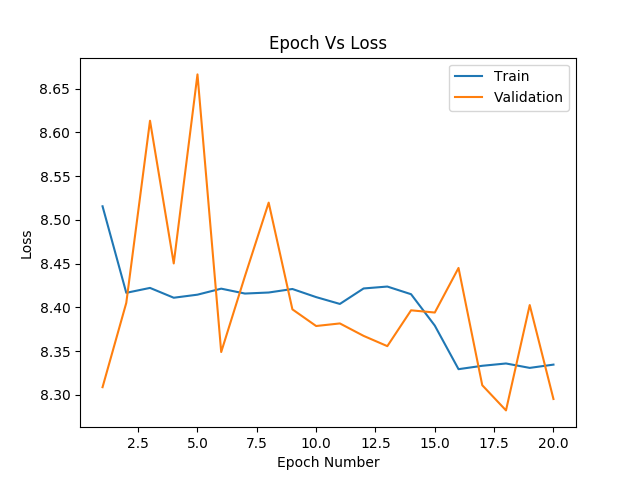
\includegraphics[width=6cm]{../Images/Epoch_VS_Loss/Sigmoid_MSE_01.png}
					\captionsetup{justification=centering,margin=1cm}
					\caption{Sigmoid, MSE, lr = 0.1.}
					\label{fig:sub1}
				\end{subfigure}%
				\begin{subfigure}{5.5cm}
					\centering
					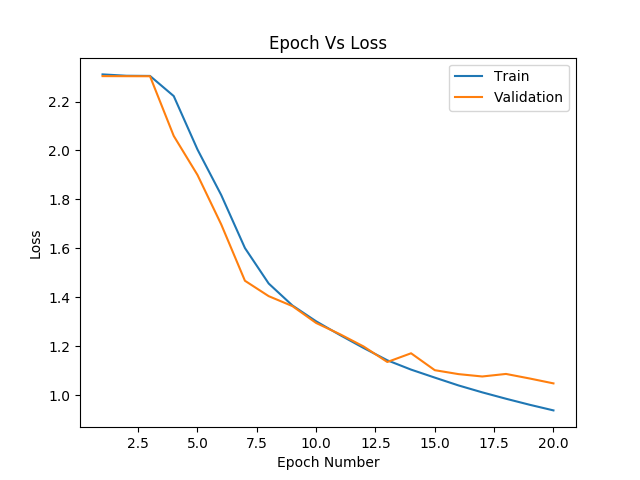
\includegraphics[width=6cm]{../Images/Epoch_VS_Loss/Sigmoid_cross-entropy_01.png}
					\captionsetup{justification=centering,margin=0.8cm}
					\caption{Sigmoid, Cross-entropy, lr = 0.1.}
					\label{fig:sub2}
				\end{subfigure}%
			
				\begin{subfigure}{5.5cm}
					\centering
					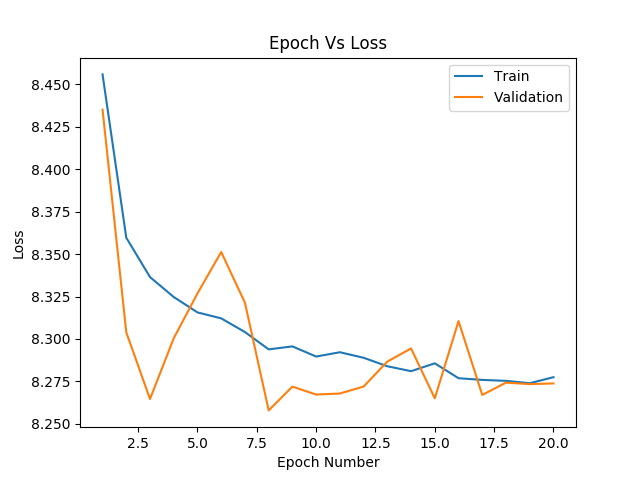
\includegraphics[width=6cm]{../Images/Epoch_VS_Loss/Sigmoid_MSE_001.png}
					\captionsetup{justification=centering,margin=1cm}
					\caption{Sigmoid, MSE, lr = 0.01.}
					\label{fig:sub3}
				\end{subfigure}
				\begin{subfigure}{5.5cm}
					\centering
					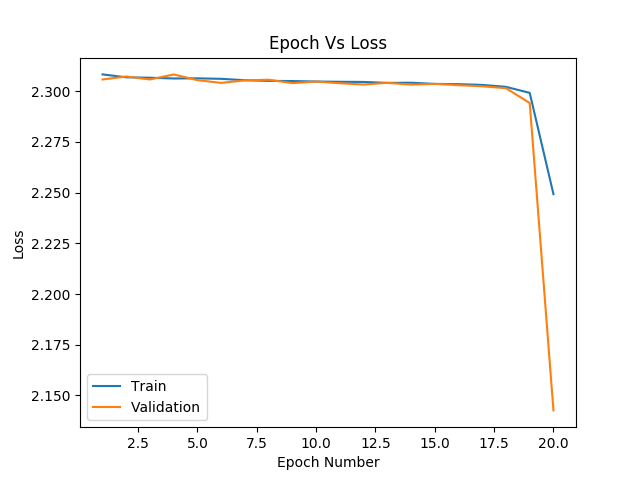
\includegraphics[width=6cm]{../Images/Epoch_VS_Loss/Sigmoid_cross-entropy_001.png}
					\captionsetup{justification=centering,margin=0.6cm}
					\caption{Sigmoid, Cross-entropy, lr = 0.01.}
					\label{fig:sub4}
				\end{subfigure}%
			
				\begin{subfigure}{5.5cm}
					\centering
					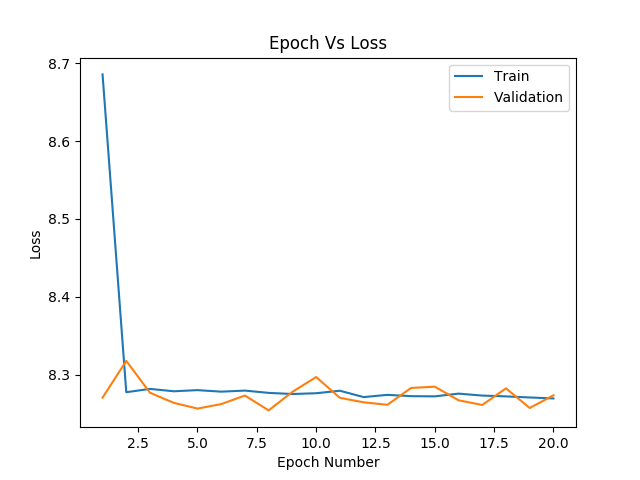
\includegraphics[width=6cm]{../Images/Epoch_VS_Loss/Sigmoid_MSE_0001.png}
					\captionsetup{justification=centering,margin=1cm}
					\caption{Sigmoid, MSE, lr = 0.001.}
					\label{fig:sub5}
				\end{subfigure}%
				\begin{subfigure}{5.5cm}
					\centering
					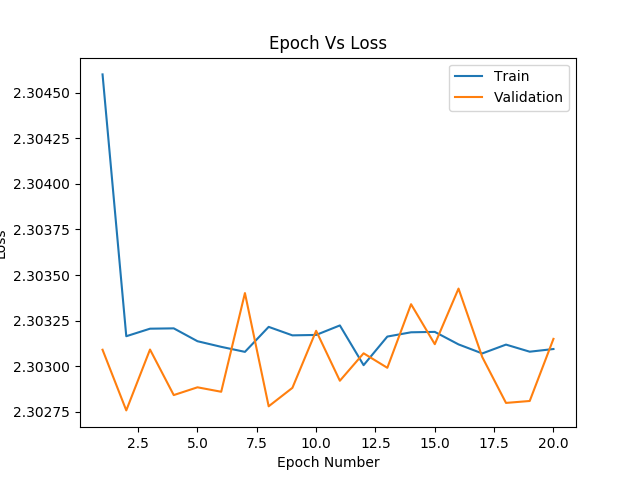
\includegraphics[width=6cm]{../Images/Epoch_VS_Loss/Sigmoid_cross-entropy_0001.png}
					\captionsetup{justification=centering,margin=0.4cm}
					\caption{Sigmoid, Cross-entropy, lr = 0.001.}
					\label{fig:sub6}
				\end{subfigure}	
				\end{framed}
				\captionsetup{justification=centering,margin=1cm}
				\caption{Experiments with the Sigmoid Activation Function}
				\label{Fig_1}
			\end{figure}
			\begin{figure}
				\centering
				\begin{framed}
				\begin{subfigure}{5.5cm}
					\centering
					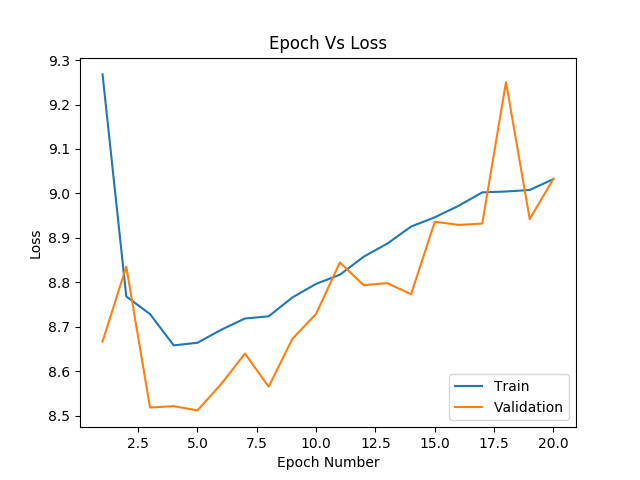
\includegraphics[width=6cm]{../Images/Epoch_VS_Loss/Tanh_MSE_01.png}
					\captionsetup{justification=centering,margin=1cm}
					\caption{Tanh, MSE, lr = 0.1.}
					\label{fig:sub7}
				\end{subfigure}
				\begin{subfigure}{5.5cm}
					\centering
					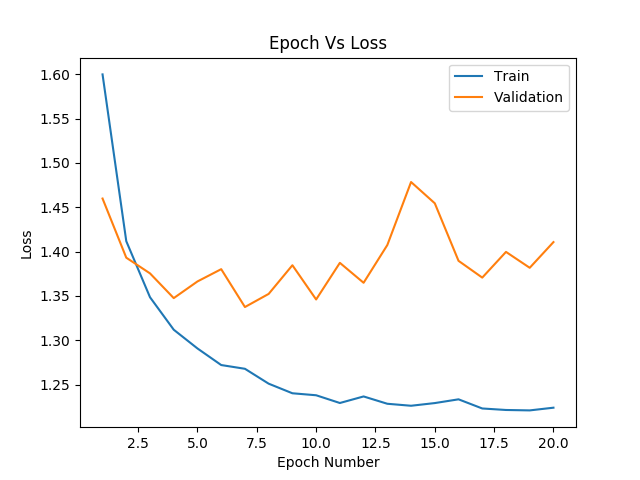
\includegraphics[width=6cm]{../Images/Epoch_VS_Loss/Tanh_cross-entropy_01.png}
					\captionsetup{justification=centering,margin=.8cm}
					\caption{Tanh, Cross-entropy, lr = 0.1.}
					\label{fig:sub8}
				\end{subfigure}
			
				\begin{subfigure}{5.5cm}
					\centering
					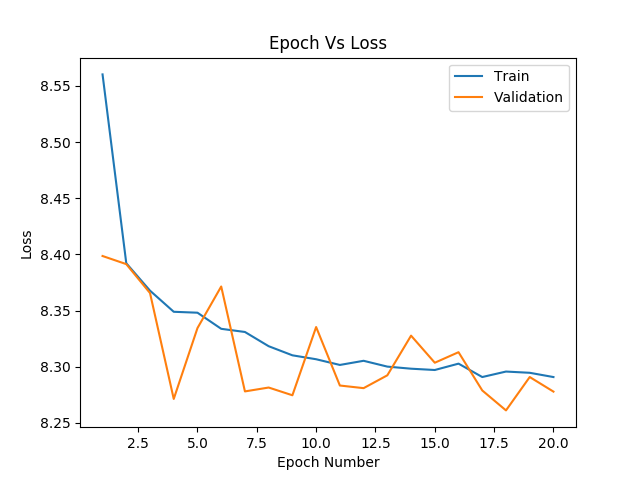
\includegraphics[width=6cm]{../Images/Epoch_VS_Loss/Tanh_MSE_001.png}
					\captionsetup{justification=centering,margin=1cm}
					\caption{Tanh, MSE, lr = 0.01.}
					\label{fig:sub9}
				\end{subfigure}
				\begin{subfigure}{5.5cm}
					\centering
					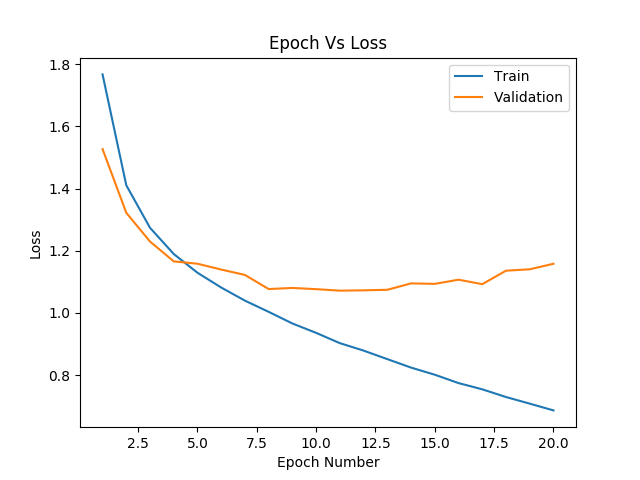
\includegraphics[width=6cm]{../Images/Epoch_VS_Loss/Tanh_cross-entropy_001.png}
					\captionsetup{justification=centering,margin=.6cm}
					\caption{Tanh, Cross-entropy, lr = 0.01.}
					\label{fig:sub10}
				\end{subfigure}%
			
				\begin{subfigure}{5.5cm}
					\centering
					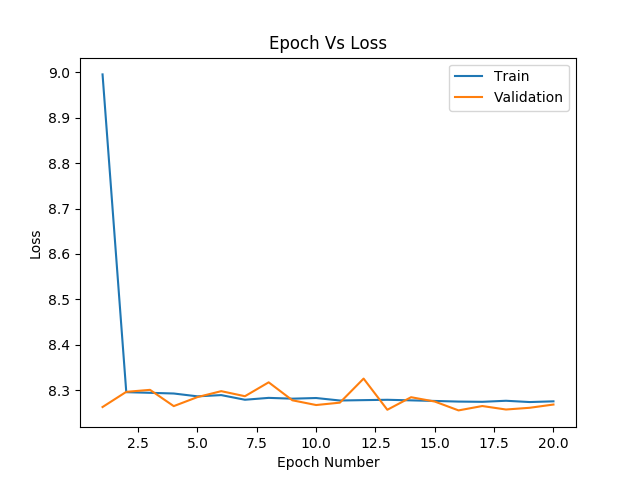
\includegraphics[width=6cm]{../Images/Epoch_VS_Loss/Tanh_MSE_0001.png}
					\captionsetup{justification=centering,margin=1cm}
					\caption{Tanh, MSE, lr = 0.001.}
					\label{fig:sub11}
				\end{subfigure}%
				\begin{subfigure}{5.5cm}
					\centering
					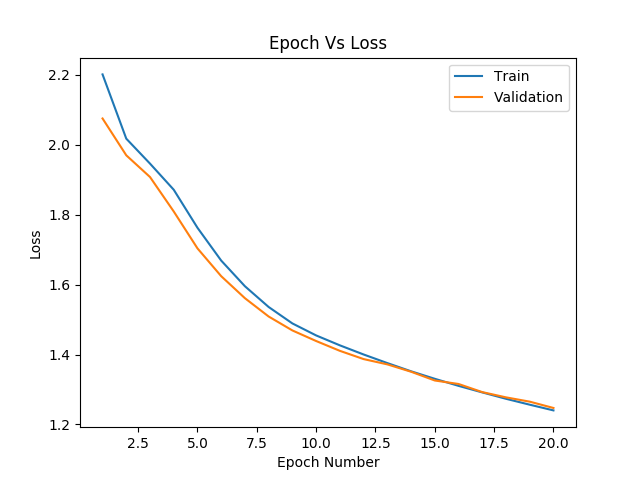
\includegraphics[width=6cm]{../Images/Epoch_VS_Loss/Tanh_cross-entropy_0001.png}
					\captionsetup{justification=centering,margin=0.4cm}
					\caption{Tanh, Cross-entropy, lr = 0.001.}
					\label{fig:sub12}
				\end{subfigure}	
				\end{framed}
				\captionsetup{justification=centering,margin=1cm}
				\caption{Experiments with the Tanh Activation Function}
				\label{Fig_2}
			\end{figure}
		
		\newpage
		\subsection{Feature Maps of 10 Images at the Last Convolution Layer}
			\begin{figure}[h]
				\centering
				\frame{
					\newline
					\begin{subfigure}{1.3cm}
						\centering
						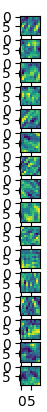
\includegraphics[width=1.3cm]{../Images/Feature_Maps_Cropped/image_0.png}
						\captionsetup{justification=centering,margin=1cm}
					%\caption{Tanh, MSE, lr = 0.1.}
					\end{subfigure}
					\begin{subfigure}{1.3cm}
						\centering
						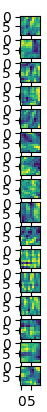
\includegraphics[width=1.3cm]{../Images/Feature_Maps_Cropped/image_1.png}
						\captionsetup{justification=centering,margin=.8cm}
						%\caption{Tanh, Cross-entropy, lr = 0.1.}
					\end{subfigure}			
					\begin{subfigure}{1.3cm}
						\centering
						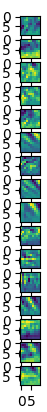
\includegraphics[width=1.3cm]{../Images/Feature_Maps_Cropped/image_2.png}
						\captionsetup{justification=centering,margin=1cm}
						%\caption{Tanh, MSE, lr = 0.01.}
					\end{subfigure}
					\begin{subfigure}{1.3cm}
						\centering
						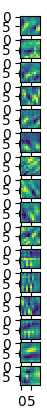
\includegraphics[width=1.3cm]{../Images/Feature_Maps_Cropped/image_3.png}
						\captionsetup{justification=centering,margin=.6cm}
						%\caption{Tanh, Cross-entropy, lr = 0.01.}
					\end{subfigure}%
					\begin{subfigure}{1.3cm}
						\centering
						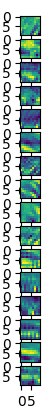
\includegraphics[width=1.3cm]{../Images/Feature_Maps_Cropped/image_4.png}
						\captionsetup{justification=centering,margin=1cm}
						%\caption{Tanh, MSE, lr = 0.001.}
					\end{subfigure}%
					\begin{subfigure}{1.3cm}
						\centering
						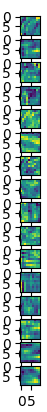
\includegraphics[width=1.3cm]{../Images/Feature_Maps_Cropped/image_5.png}
						\captionsetup{justification=centering,margin=0.4cm}
						%\caption{Tanh, Cross-entropy, lr = 0.001.}
					\end{subfigure}	
				\begin{subfigure}{1.3cm}
					\centering
					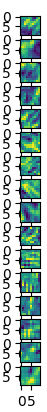
\includegraphics[width=1.3cm]{../Images/Feature_Maps_Cropped/image_6.png}
					\captionsetup{justification=centering,margin=1cm}
					%\caption{Tanh, MSE, lr = 0.01.}
				\end{subfigure}
				\begin{subfigure}{1.3cm}
					\centering
					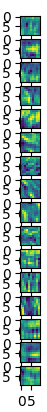
\includegraphics[width=1.3cm]{../Images/Feature_Maps_Cropped/image_7.png}
					\captionsetup{justification=centering,margin=.6cm}
					%\caption{Tanh, Cross-entropy, lr = 0.01.}
				\end{subfigure}%
				\begin{subfigure}{1.3cm}
					\centering
					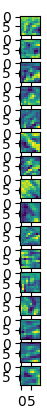
\includegraphics[width=1.3cm]{../Images/Feature_Maps_Cropped/image_8.png}
					\captionsetup{justification=centering,margin=1cm}
					%\caption{Tanh, MSE, lr = 0.001.}
					\label{fig:sub5}
				\end{subfigure}%
				\begin{subfigure}{1.3cm}
					\centering
					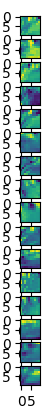
\includegraphics[width=1.3cm]{../Images/Feature_Maps_Cropped/image_9.png}
					\captionsetup{justification=centering,margin=0.4cm}
					%\caption{Tanh, Cross-entropy, lr = 0.001.}
				\end{subfigure}	
				}
				\captionsetup{justification=centering,margin=1cm}
				\caption{Feature maps of 10 images at the last convolution layer. Parameters = (b\_size = 10, activation function = Tanh, loss function = cross-entropy, l\_r = 0.01).}
				\label{fig_3}
			\end{figure}
		
		From Figure \ref{fig_3}, we can see that our network has already learned $16*5*5 = 400$ features for each image after the second convolutional layer. The network used corresponds to the one in figure \ref{fig:sub10}.
		
		\newpage
		\section{Select Relu, Learning Rate of 0.001, Cross-entropy Loss. Change the Network to Use 3x3 Kernels}
			\begin{figure}[h]
				\centering
				\begin{framed}
					\centering
					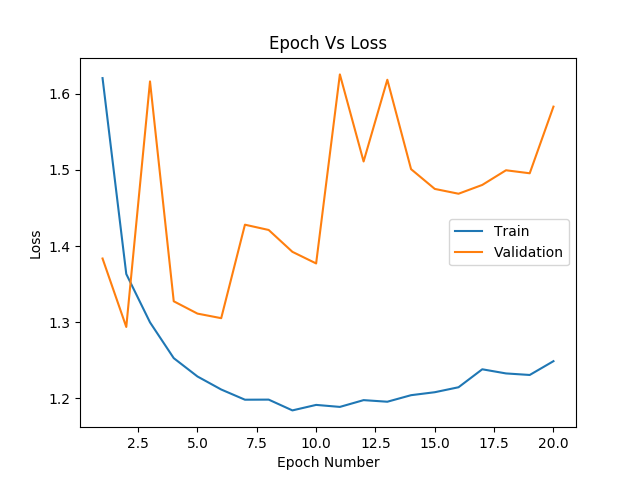
\includegraphics[width=12cm]{../Images/Epoch_VS_Loss/ReLU_cross-entropy_01.png}
					\captionsetup{justification=centering,margin=1cm}
				\end{framed}
					\caption{Relu, cross-entropy, lr = 0.001, 3x3 kernels.}
					\label{Fig_4}
			\end{figure}
		
			In terms of classification accuracy, the previous network (figure \ref{fig:sub10}) achieved 62\% while the current one (figure \ref{Fig_4}) achieved 51\%. When looking at the loss curves, we can see that at epoch 20, the previous network is still learning while the current one seems to have stopped learning at epoch 7. This can explain why the previous network produced better accuracy results.
		
		\newpage
		\section{Build a CNN with 5 Convolution Layers with 3x3 Kernels and Corresponding 2x2 Average Pooling with Stride 1}
		\subsection{How long did it take to train? Why?}
		
			It took 1h13 mins to train and the reason why it took so long is because by using padding and decreasing the kernel size and pooling stride, the size of the image does not change by much after each convolution block (convolution layer + pooling layer) which still leaves a large number of parameters to be trained after each block. Then by increasing the number of convolution blocks, the number of parameters to be trained exploded.
			
		\subsection{How does the Accuracy of this Network Compare Against the Previous Two? Explain}
			This network produced an accuracy of 61\% compared to 62\% and 51\% respectively for the previous two networks (figures \ref{fig:sub10} and \ref{Fig_4}). However, when looking at the loss curves, we can see that for this network, the training loss gets close to 0 at epoch 50 while the test loss seems to be increasing. This can be a proof that the network has over-fitted the training dataset. One cause could be that the number of parameters trained is way larger than what is necessary to solve this kind of problem.
			\begin{figure}[h]
				\centering
				\begin{framed}
					\centering
					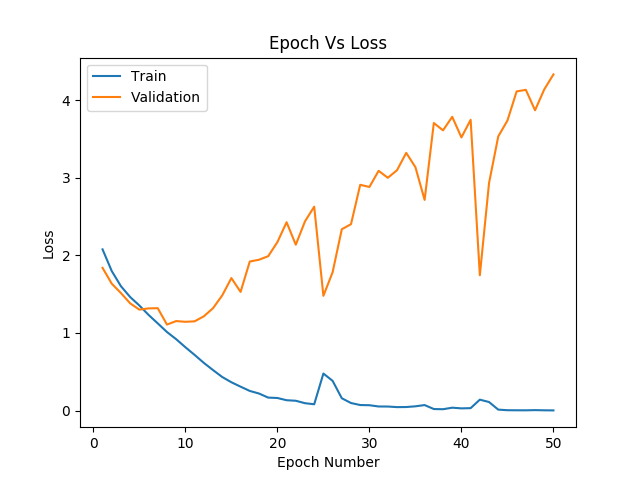
\includegraphics[width=12cm]{../Images/Epoch_VS_Loss/ReLU_5_conv_cross-entropy_01.png}
					\captionsetup{justification=centering,margin=1cm}
				\end{framed}
				\caption{5 Convolution Layers, Relu, cross-entropy, lr = 0.1, 3x3 kernels, 2x2 average pooling (stride = 1).}
				\label{Fig_5}
			\end{figure}
		
		
	%\bibliographystyle{ieeetr}
	%\bibliography{references}
	
\end{document}
